
% Cal Poly Thesis
% 
% based on UC Thesis format
%
% modified by Mark Barry 2/07.
%




\documentclass[12pt]{ucthesis}

%\newif\ifpdf
%\ifx\pdfoutput\undefined
%    \pdffalse % we are not running PDFLaTeX
%\else
%\pdfoutput=1 % we are running PDFLaTeX
%\pdftrue \fi

\usepackage{textcomp}
\usepackage{url}
\usepackage{listings}
\lstset{
	language=[Visual]C++,
	keywordstyle=\bfseries\ttfamily\color[rgb]{0,0,1},
	identifierstyle=\ttfamily,
	commentstyle=\color[rgb]{0.133,0.545,0.133},
	stringstyle=\ttfamily\color[rgb]{0.627,0.126,0.941},
	showstringspaces=false,
	basicstyle=\small,
	numberstyle=\footnotesize,
	numbers=left,
	stepnumber=1,
	numbersep=10pt,
	tabsize=2,
	breaklines=true,
	prebreak = \raisebox{0ex}[0ex][0ex]{\ensuremath{\hookleftarrow}},
	breakatwhitespace=false,
	aboveskip={1.5\baselineskip},
  columns=fixed,
  upquote=true,
  extendedchars=true
% frame=single,
% backgroundcolor=\color{lbcolor},
}
\usepackage{color}
%\ifpdf

    \usepackage[pdftex]{graphicx}
    % Update title and author below...
    \usepackage[pdftex,plainpages=false,breaklinks=true,colorlinks=true,urlcolor=blue,citecolor=blue,%
                                       linkcolor=blue,bookmarks=true,bookmarksopen=true,%
                                       bookmarksopenlevel=3,pdfstartview=FitV,
                                       pdfauthor=Christopher Gibson,
                                       pdftitle=Point-Based Color Bleeding With Volumes,
                                       pdfkeywords={thesis, masters, cal poly, volume rendering, global illumination}
                                       ]{hyperref}
    %Options with pdfstartview are FitV, FitB and FitH
    \pdfcompresslevel=1

%\else
%    \usepackage{graphicx}
%\fi

\usepackage{amssymb}
\usepackage{amsmath}
\usepackage[letterpaper]{geometry}
\usepackage[overload]{textcase}



%%%%%\bibliographystyle{abbrv}

\setlength{\parindent}{0.25in} \setlength{\parskip}{6pt}

\geometry{verbose,nohead,tmargin=1.25in,bmargin=1in,lmargin=1.5in,rmargin=1.3in}

\setcounter{tocdepth}{2}


% Different font in captions (single-spaced, bold) ------------
\newcommand{\captionfonts}{\small\bf\ssp}

\makeatletter  % Allow the use of @ in command names
\long\def\@makecaption#1#2{%
  \vskip\abovecaptionskip
  \sbox\@tempboxa{{\captionfonts #1: #2}}%
  \ifdim \wd\@tempboxa >\hsize
    {\captionfonts #1: #2\par}
  \else
    \hbox to\hsize{\hfil\box\@tempboxa\hfil}%
  \fi
  \vskip\belowcaptionskip}
\makeatother   % Cancel the effect of \makeatletter
% ---------------------------------------

\begin{document}

% Declarations for Front Matter

% Update fields below!
\title{Point-Based Color Bleeding With Volumes}
\author{Christopher Gibson}
\degreemonth{June} \degreeyear{2011} \degree{Master of Science}
\defensemonth{June} \defenseyear{2011}
\numberofmembers{3} \chair{Zo\"{e} Wood, Ph.D.} \othermemberA{Aaron Keen, Ph.D.} \othermemberB{Chris Lupo, Ph.D.} \field{Computer Science} \campus{San Luis Obispo}
\copyrightyears{seven}



\maketitle

\begin{frontmatter}

% Custom made for Cal Poly (by Mark Barry, modified by Andrew Tsui).
\copyrightpage

% Custom made for Cal Poly (by Andrew Tsui).
\committeemembershippage

\begin{abstract}

The interaction of light in our world is immensely complex, but with modern computers and advanced rendering algorithms, we are beginning to reach the point where photo-realistic renders are truly difficult to separate from real photographs.  Achieving realistic or believable global illumination in scenes with participating media is exponentially expensive compared to our traditional polygonal methods.  Light interacts with the particles of a volume, creating complex radiance patterns.

In this thesis, we introduce an extension to the commonly used point-based color bleeding (PCB) technique, implementing volume scatter contributions.  With the addition of this PCB algorithm extension, we are able to render fast, believable in- and out-scattering while building on existing data structures and paradigms.  The proposed method achieves results comparable to those produced with Monte Carlo ray tracing but with drastically reduced run times, speeding up renders by nearly a factor of 10.

We present results that are both comparable to existing Monte Carlo integration methods while also achieving much faster run-times with minimal memory usage.

\end{abstract}

%\begin{acknowledgements}

%   Thank you...

%\end{acknowledgements}


\tableofcontents


\listoftables

\listoffigures

\end{frontmatter}

\pagestyle{plain}




\renewcommand{\baselinestretch}{1.66}


% ------------- Main chapters here --------------------





\chapter{Introduction}
\label{intro}

\section{Graphics \& Light}
At its core, computer graphics is the visualization of light and its interaction in an abstract world, be this a simulation or a virtual world created by artists.  The ability to render scenes with realistic lighting is desirable for many entertainment application settings such as film.  Even in non-photo-realistic renders, the interaction of light is of paramount importance.

\section{Global Illumination}
The effort to accurately evaluate the radiometric quantities within a virtual scene, especially in non-real-time systems, may be referred to collectively as \textit{global illumination} \cite{verth:2008}.  In order to achieve greater realism, scenes must rely on more than simple direct-lighting algorithms and move to more complex systems to better evaluate light interaction (Figure \ref{fig:cornell}.)  This field of study has lent itself to the breathtaking visual effects in movies, advertisements, television shows and other artistic mediums.  The line between real and fake is getting blurrier every year as the lighting calculations become more and more exact.  As we have pushed the boundaries of our graphical capabilities, we also increase our computational complexity exponentially.

\begin{figure}[h!]
    \centering
    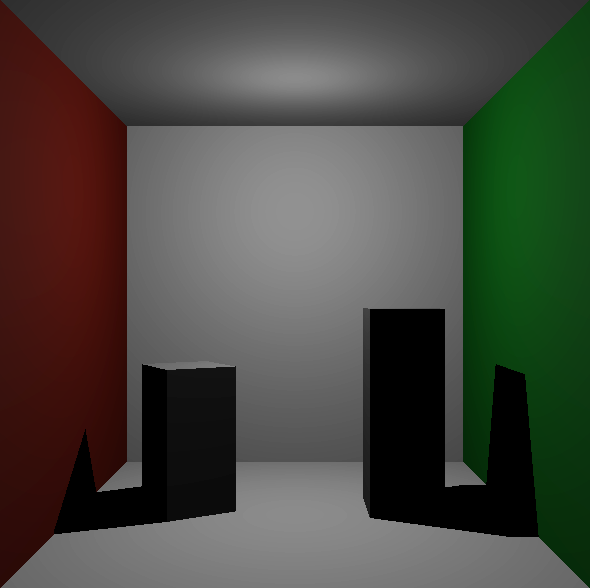
\includegraphics[width=70mm]{img/boxes_noindirect.png}
    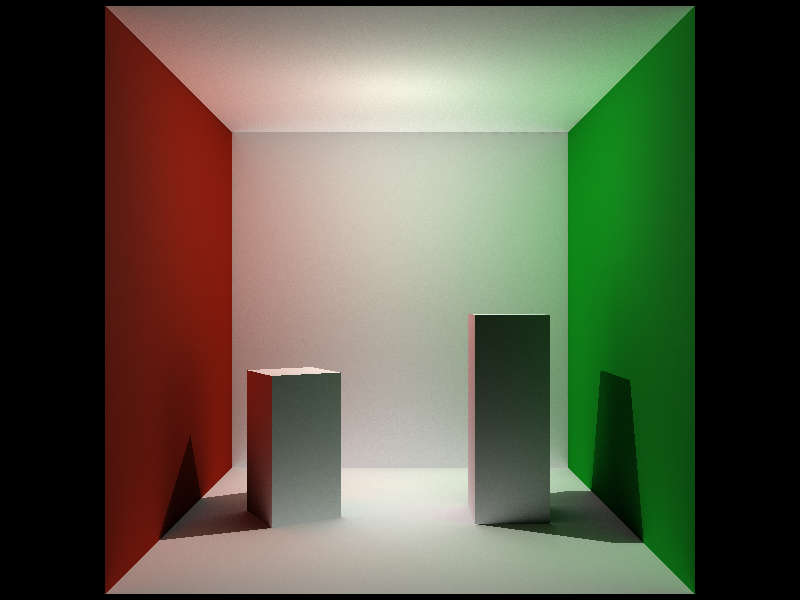
\includegraphics[width=70mm]{img/indirect_box_high.png}
    \captionfonts
    \caption{A simple Cornell box scene with direct lighting only (left) and the same scene showing single-bounce light interaction through a global illumination algorithm (right.)}
    \label{fig:cornell}
\end{figure}

\section{Color Bleeding Techniques}

Great results have been achieved for lighting complex scenes using point based color bleeding~\cite{christensen:2008} algorithms, where a point-cloud representation of a scene's direct lighting is computed for the purpose of efficiently calculating a representation of the scene's radiometric properties surrounding any given point.  Per H. Christensen's color bleeding algorithm (or similar implementations) is already in place in many production companies and used in many feature films.

These algorithms, however, tend to limit or omit entirely the lighting contribution from volumetric data or participating media within the scenes.  Due to the highly complex nature of the domain, coupled with the computational complexity involved therein, many algorithms choose to disregard this portion of the lighting algorithm, often leaving the programmer or artist to fake the volume's contribution in other ways.


\section{Our Contribution}

This paper presents an algorithm to address this missing component in the point based color bleeding algorithm.  Specifically, we propose the addition of a data representation tuned to volumes,  \emph{light-voxel (or lvoxel)} to address the need to represent participating media to an existing global illumination algorithm which leverages a point cloud representation of a scene.  Over the course of this paper, we will:

\begin{enumerate}
\item Discuss the surrounding subjects of light, volume rendering and global illumination,
\item List and describe the seminal and related works,
\item Describe how our algorithm meets our requirements and
\item Analyze the results of our implementation.
\end{enumerate}

Our method achieves results comparable to those produced with Monte Carlo ray tracing but with drastically reduced run times, speeding up renders by a factor of 10.  Figure~\ref{fig:compare} clearly illustrates a close comparison of our algorithm and Monte Carlo ray traced results.

\begin{figure}[h!]
    \centering
    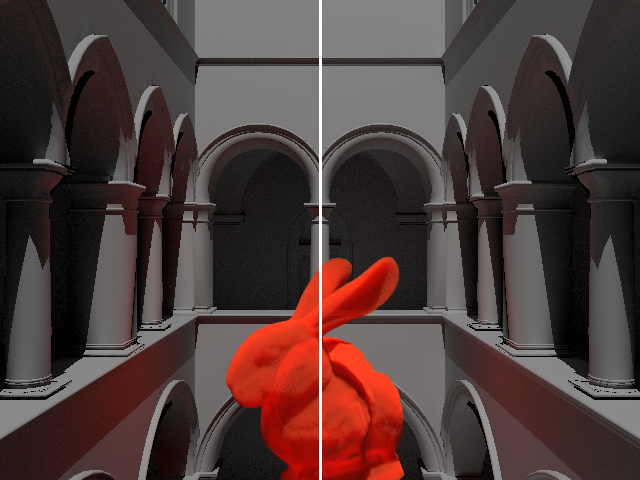
\includegraphics[width=100mm]{img/compare.png}
    \caption{Comparison of the PCB extension (left) and traditional Monte Carlo results (right.)}
    \label{fig:compare}
\end{figure}

\chapter{Background}
\label{background}

The goal of the proposed method is to include volumetric representations into a global illumination algorithm in a fast and coherent way. One of the unique features of participating media is that they must be represented with a more complex data-structure than solid geometric objects which are usually polygonalized in most rendering processes.  Light interacts with the particles of a volume, creating complex radiance patterns (increasing the necessary computational complexity exponentially.) In particular the most fundamental concepts are presented here,  (based off of  \cite{pbrt}).

%----------------------------------%
\section{Radiance}

\begin{figure}[h!]
    \centering
    \includegraphics[width=80mm]{img/diag/radiance.pdf}
    \captionfonts
    \caption{Evaluation of radiance at a point on an opaque surface.  Only the hemisphere around the surface normal is considered.  Incoming radiance is measured and scaled by its solid angle.}
    \label{fig:radiance}
\end{figure}

Irradiance is the change of flux (radiant power) over an area, denoted by $E = \frac{d\Phi}{dA}$ \cite{aga}. Another way to look at this problem involves the relationship between the surface and surrounding radiometric quantities.  Radiance helps us evaluate how much power enters or leaves any given point.  The definition of radiance leaving a surface can be denoted $L(\textup{p}, w)$ given $\textup{p}$ is the point on a surface and $w$ is the direction we are evaluating.  The flux is projected upon the area of the surface $dA$ based on the solid angle $dw$, which gives us Figure \ref{fig:radiance} and the following equation:

\begin{equation}
\mathit{L} = \frac{\mathit{d^{2}\Phi}}{\mathit{dwdA}^\perp}
\label{eq:radiance}
\end{equation}

Inversely, incoming radiance, or irradiance, is evaluated by the strength of the light coming from any given direction $w$.  This  can be represented by the following:

\begin{equation}
\mathit{E} = \int\mathit{L}(\textup{p} \leftarrow w)\textup{cos}\theta dw.
\label{eq:irradiance}
\end{equation}

$\mathit{L}(\textup{p} \to w)$ represents the radiance leaving point $\textup{p}$ and $\mathit{L}(\textup{p} \leftarrow w)$ represents incoming radiance given a direction $w$.  Note that radiance along a straight path is invariant.  For example:

\begin{equation}
L(x \to y) = L(y \to x).
\label{eq:invariance}
\end{equation}

Measuring the incoming radiance at any given point $\textup{p}$ in all directions is the key to the graphics lighting equation, and a crucial element in how a rendered scene looks and feels.

\section{BRDF and the BSRDF}

The \textit{bidirectional reflectance distribution function} (or BRDF) is a function that gives us a formal method of describing the reflected radiance from a surface given an incident radiance from another light source or emissive surface \cite{brdf}.  This simplification helps us with quick evaluations in scenes with simple lighting (such as point light sources) and other direct-lighting techniques.  The BRDF can be generalized into the following equation, based off of Equation \ref{eq:irradiance}.  If the incident direction $w_{i}$ represents the differential cone of incoming directions, the differential radiance at point $\textup{p}$ is represented by:

\begin{equation}
\textup{d}\mathit{E}(\textup{p}, w_{i}) = \mathit{L}_{i}(\textup{p}, w_{i})\textup{cos}\theta_{i} \textup{d}\mathit{w_{i}}.
\label{eq:brdf}
\end{equation}


Many materials such as skin, marble and plastic do not simply reflect the incoming light energy, but also transmit it through the surface, a process called \textit{subsurface scattering}.  Given the obvious shortfalls of the BRDF in this instance, the BSRDF (\textit{bidirectional scattering-surface reflectance distribution function}) takes into account a surface's scatter properties.  This generalized function describes the ratio of "" differential radius from incoming point and direction $\textit{p}_{i}$, $w_{i}$ to an outgoing point and direction $\textit{p}_{i}$, $w_{o}$.  This turns a one-dimensional reflectance equation into a two-dimensional scatter equation, significantly increasing its complexity.

\section{Volume Lighting}

The BSSRDF describes the complexities of light traveling and scattering within complex surfaces similarly to that of volumes.  Volumes follow very similar behaviors to opaque surfaces in terms of radiance, except on a particle-level.  Participating media like smoke or fog is made up of particles which cause the scatter (i.e. clouds) and absorption/extinction (i.e. smoke,) behaviors that would be extremely computationally expensive to model and simulate on any scale.  Therefore, such behaviors are modeled in terms of transmittance, emission, Scatter in and Scatter out like in Figure \ref{fig:vol_scat}.  We are able to identify the probability that light will be absorbed, scattered and/or transmitted through any point in a participating medium by identifying their probability density functions, as described in the following sections. 
\begin{figure}[h!]
    \centering
    \includegraphics[width=100mm]{img/diag/vol_scatter.pdf}
    \captionfonts
    \caption{Light scatter properties vary based on the participating media.}
    \label{fig:vol_scat}
\end{figure}

%----------------------------------%
\subsection{Absorption:}
As light passes through a participating media, light will become absorbed based on its absorption probability density $\sigma_{a}$. As stated earlier in Equation \ref{eq:invariance}, it is known that radiance along a straight path is invariant, which allows us to estimate the amount of light absorbed or scattered given point $p$ and direction $w$ with the following:

\begin{equation}
e^{-\int_{0}^{d}\sigma_{a} (p+t\mathit{w},\mathit{w})d\mathit{t}},
\label{siga_eq}
\end{equation}

where $\sigma_{a}$ represents the probability density that light will be absorbed over a distance $\textup{d}\mathit{t}$.

%----------------------------------%
\subsection{Scatter Out:}
In addition to being absorbed by the medium, light can be scattered based on a scatter probability density $\sigma_{s}$.  As light is scattered and thus redirected, the amount of energy passing through the density in direction $w$ is reduced.  We can model the scatter equation through the following equation:

\begin{equation}
\textup{d}\mathit{L}_{o}(\textup{p},w) = -\sigma_{s}(\textup{p},w) \mathit{L}_{i}(\textup{p},-w)\textup{d}t.
\label{sigs_eq}
\end{equation}

$\textup{d}L_{o}$ represents the outgoing radiance given point $\textup{p}$ and direction $w$.

%----------------------------------%
\subsection{Transmittance:}
Both (\ref{siga_eq}) and (\ref{sigs_eq}) involve the reduction of energy through a volume, reducing how much energy passes through (also known as its transmittance.)  The two can be combined into the following overarching representation:

\begin{equation}
\sigma_{t}(\textup{p},w) = \sigma_{a}(\textup{p},w) + \sigma_{s}(\textup{p}, w).
\label{eq:sigt}
\end{equation}

Equation \ref{eq:sigt} gives us transmittance ($\sigma_{t}$) at point $\textup{p}$ and direction $w$.  Using this representation, we can integrate over a ray passing through the volume in order to evaluate the resulting radiance transmittion:

\begin{equation}
T_{r}(\textup{p} \to \textup{p}') = e^{-\int_{0}^{d}\sigma (p+t\mathit{w},\mathit{w})d\mathit{t}}.
\label{transmittion_eq}
\end{equation}

%----------------------------------%
\subsection{Phase Functions}

\begin{figure}[h!]
    \centering
    \includegraphics[width=80mm]{img/diag/phase_func.pdf}
    \captionfonts
    \caption{Visual representation of a phase function around a scatter point.  The area represents the distribution of the scattered light about a sphere.}
    \label{fig:phase}
\end{figure}

When dealing with particles in volumes that may scatter light, a distribution function or \textit{phase function} describes the angular distribution of light scattered, described as $phase(w \to w')$.  The probability that light may scatter from direction $w$ to $w'$ is described using this function.  This distribution is visualized in Figure \ref{fig:phase}. All tests in this paper were rendered using one of the simplest phase functions, known as the isotropic or \textit{constant} phase function which represents the BRDF analog for participating media \cite{cerezo}.


%----------------------------------%
\subsection{Scatter In}
Although $\sigma_{s}$ may reduce the energy of a ray passing through a volume, radiance from other rays (scattered by their respective phase functions as seen in Figure \ref{fig:phase}) may contribute to the original ray's radiance.  This allows for radiance emitted from surrounding participating media and geometry to contribute to any given point within the volume, as exemplified in Figure \ref{fig:inscat}.  Before we can integrate incoming radiance, we must take into account the \textit{source term} $\mathbb{S}$, or total added radiance per unit distance, where the following constraint must hold true:

\begin{equation}
\int_{\mathbb{S}^2}phase(w \to w')\textup{d}w' = 1.
\label{eq:source}
\end{equation}

This normalization makes sure that the phase function accurately defines the probability distribution for a particular direction.  Given a summation of all outgoing radiance along every direction $w'$, we should be left with the total incoming radiance from direction $w$.

\begin{figure}[h!]
    \centering
    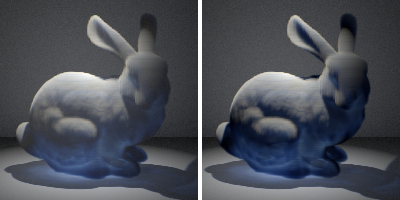
\includegraphics[width=80mm]{img/inscat_comp.png}
    \captionfonts
    \caption{Comparison between a volume with (right) and without (left) in-scattering contribution.}
    \label{fig:inscat_comp}
\end{figure}

Finally, assuming conditions are met for Equation \ref{eq:source}, we can integrate the total radiance scatter based on the normalized phase function $phase(w \to w')$ over all directions $w'$ to get our total scatter in a direction $w$:

\begin{displaymath}
\mathit{S}(\textup{p},w) = \mathit{L}_{\textup{ve}}(\textup{p},w) + \sigma_{\textup{s}}(\textup{p}, w) \int_{\mathbb{S}^2} phase(\textup{p}, -w' \to w) L_{i}(\textup{p},w')\textup{d}w'.
\end{displaymath}

$L_{\textup{ve}}(\textup{p}, w)$ represents the emission coefficient of a volume and is not discussed in this paper.


\section{Monte Carlo Integration}

Monte Carlo methods have many applications in estimating complex systems through the use of random numbers and sampling schemes.  One of the most useful technique is Monte Carlo integration, which estimates the integral of an arbitrary function through sampling discrete values defined over a specified domain \cite{aga}.  For this reason, Monte Carlo has become \textit{integral} in the field of computer graphics, where it may manifest itself in evaluating incoming radiance over a surface, estimating light scatter, or randomly sampling area lights in order to get soft shadows.

Many of the elements listed above can be (and are) estimated using this technique.  In order to get good results, however, many hundreds of samples may be necessary.  The cost of sampling using this method may still be cost-prohibitive, at which point the problem lies in the sample method itself, not how the samples are used or generated.

\chapter{Related Work}

\section{Global Illumination}
Global illumination is an important field of study in computer graphics that numerous successful algorithms including photon mapping \cite{Jensen:2009}, radiosity \cite{radiosity} and Monte Carlo sampling techniques \cite{monte_carlo} try to mitigate or overcome in a reasonable time-frame.  Most commonly implemented methods are those that sample the scene and use a two phase approach (sample and gather) to model direct illumination and indirect illumination.  The gather stage included in most algorithms is built to be more efficient or lower resolution than the scene being rendered, which helps cut down severely on the lighting computation cost.

\subsection{PCB}
Of particular relevance to this field is the work done in Point-Based Approximate Color Bleeding developed by Per Christensen \cite{christensen:2008}.  With this method, a subset of the scene geometry is thoroughly sampled, creating a point cloud representation of the direct lighting at each sample, which is then used to evaluate the incoming radiance surrounding a given point on a surface.

As recently as 2010, discussion of approximating volume scattering using point clouds has been discussed \cite{christensen:siggraph}, however no specifics have been offered to how \textit{back-to-front or front-to-back rasterization} would be achieved with the current rasterization method (handled by our octree traversal method) or how scatter, extinction and absorption would be managed within the three-dimensional volume representation inside the point cloud.

\subsection{Photon Mapping}
Another closely related area of study includes photon mapping, a method that attempts to simulate light scatter and absorption properties of participating media, which has shown promise in the past.  In \cite{jensen:1998}, Jensen describes a process where photons participate and become stored inside the volume itself for later gathers during volume integration.  These photons are able to simulate scatter, absorption and passing through material (both geometric and volumetric.)

While this technique is shown to work, it primarily focuses on caustic effects in volumes and the generated photon map.  Our storage method does not require data to be stored in the volume itself (as would be the case in photon mapping,) but in a separate, more lightweight data-structure better suited for out-of-core rendering.

\begin{figure}[h!]
    \centering
    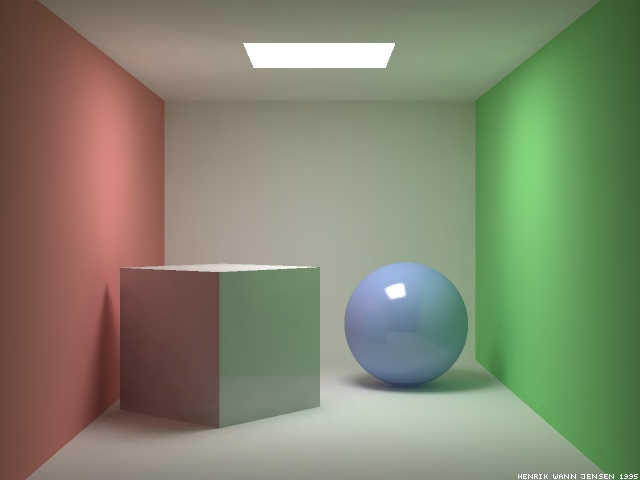
\includegraphics[width=100mm]{img/external/ewr7_mcbox.jpg}
    \caption{Global illumination example achieved via photon mapping.  Source: http://graphics.ucsd.edu/\string~henrik/papers/photon\_map/}
    \label{fig:photon}
\end{figure}

\section{Volume Rendering}
This paper is focused on the lighting and rendering of scenes which contain volume data.  A number of approaches have been developed in order to represent volume data through computer visualizations or renders~\cite{levoy88}\cite{Kajiya84}.

\subsection{Seminal Work}
Some of the first proposed volume rendering and shading techniques are described in \cite{levoy88}.  Before the time of the paper's creation, many of the accepted methods of volume visualization involved generating polygonal representations of the volumes by sampling the opacities and comparing them to a selected isovalue to determine whether or not the voxel is designated as "inside" the volume or "outside."  A polygonal mesh is then constructed based on this differentiating boundary.  Unfortunately, the algorithm defined above fell prey to spurious surfaces and holes caused by a limited sample range (since the polygonal method suffered from having to make a binary decision.  Either a ray intersected the volume or it did not.)

In response to this, Levoy proposed a process of testing against two arrays (one with opacities and one with colors) that represent the voxel data-structure.  If a voxel was intersected, the algorithm would interpolate its color and opacity to those surrounding it based on the nature of the intersection.  This allowed for transparent volumes, and also allowed for opacities to be separated from voxel color, allowing for some important pre-processing to be done on the data such as volume classification, where the opacity of a volume determined on an iso range.  This in turn allowed the renderer to focus attention to specific densities in scans (useful for medical imaging.)

\begin{figure}[h!]
    \centering
    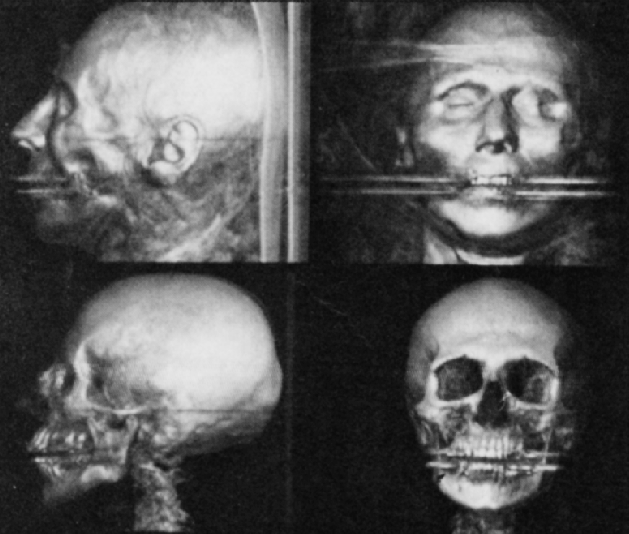
\includegraphics[width=100mm]{img/external/img188.png}
    \caption{Volume renders from \cite{levoy88} showing CT scan volume data visualized in three-dimensions, complete with realistic lighting. }
    \label{fig:levoy}
\end{figure}

\subsection{Multi-Resolution Volumes}
Because of the complexity of volume data (both through data representation and computation,) volume rendering algorithms often implement efficient multi-resolution data representation~\cite{Westermann94}.  \cite{Levoy90} describes a hierarchical method of managing a volume data set in order to remove unnecessary "Empty" cells and to reduce the amount of intersection tests done on voxels (or "Cells", as the higher level nodes are referred to.)  This algorithm introduced the use of octrees as an efficient means of dividing and containing the volume data.

Our algorithm implements a sparse octree data-structure for both the volumes in the scene and the point-cloud used for the indirect lighting equation.

\subsection{Occlusion Techniques}
Another method to accelerate volume rendering involves estimating what nodes in a volume octree are definitely occluded based on surrounding node densities.  \cite{guthe} describes building a two-dimensional occlusion map and filling it in over a series of iterations, removing occluded nodes from being tested each iteration.  This method has been shown to drastically increase rendering performance by removing as much as 30\% per iteration.

Based on many seminal volume rendering algorithms, our implementation takes advantage of a multi-resolution, view-independent octree data-structure in order to handle a large amount of complex lighting and volume data.  We then use this very same octree representation to evaluate occluded regions, skipping scene data occluded by opaque geometry cached in the data-structure in the form of surfels.

\subsection{Volume Lighting}
As our computational power has improved, we have been able to tackle problems in lighting that we could not have overcome in the past.  \cite{kniss:03} builds upon Levoy's volume rendering method by implementing shadowing by sending shadow rays toward each light for each sample within the volume in order to estimate the amount of extinction between the point and the light.  Indirect lighting is also employed (though only forward-scattering due to the incremental nature of their algorithm.)

\cite{zhang} attempts to handle multiple-scattering and volume shadows in scenes that sport mixed polygonal and volumetric data.  The paper describes light scatter representations similar to Equations \ref{siga_eq}, \ref{sigs_eq}, \ref{eq:sigt}, where light is able to scatter in and out from the sampling ray.  The algorithm then handles volume shadows caused by polygonal mesh data by constructing a series of shadow buffers, evaluating the volume shadow as a texture at each slice.

While our volume lighting equation takes into account volume scatter properties, we do not evaluate shadows in a separate pass.  Instead, our algorithm not only evaluate transmittance between arbitrary sample points and the scene lights (giving us believable direct lighting,) but we simulate scatter in properties by casting Monte Carlo samples out into our point-cloud to evaluate scene and volume radiance.  Additionally, our point cloud is not constrained by our traversal method, so all forms of scatter are supported.  Finally, the algorithm described also does not handle scatter out contributions to the scene, where the volume data may contribute to the rest of the scene's lighting.

%==============================================================================%
\chapter{PCB Extension Algorithm}
\label{algorithm_sec}
We present an algorithm which is an extension to the point cloud techniques described in \cite{tabellion} and \cite{christensen:2008}, specifically building off the point-based color bleeding (PCB) technique by Christensen.  The modifications involve evaluating light scatter and absorption properties at discrete points in the volume and adding them to the point cloud.  Using a front-to-back traversal method, we can correctly and quickly approximate the \textit{light-volume} representation's contribution to a scene's indirect lighting evaluation.

\section{Point Based Color Bleeding}

\begin{figure}[h!]
    \centering
    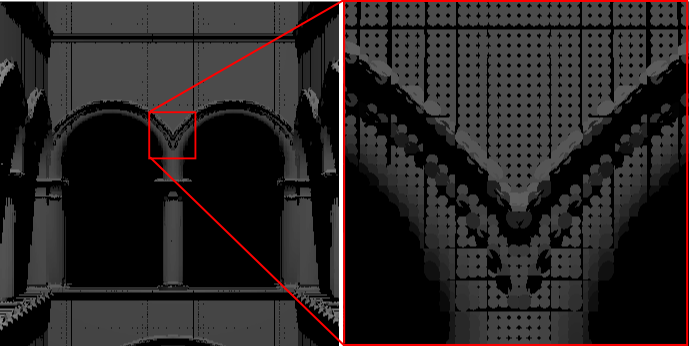
\includegraphics[width=100mm]{img/pcloud.png}
    \caption{An example of a point-cloud scene where the geometry had been sampled, a disc representation replacing the geometry.  The radii of the discs in this image are reduced to better exemplify their presence.}
    \label{fig:pcloud}
\end{figure}

In general, the color-bleeding algorithm subdivide the world into small representational segments, called surfels in \cite{christensen:2008}, which are stored in a large point cloud, representing the scene (See Figure \ref{fig:pcloud}.)  Surfels are used to model direct illumination, and are then used in a later phase to compute indirect lighting and color bleeding in an efficient manner.  This method is split up into three stages:

\begin{enumerate}
\item Sample the scene and save a discrete representation of the surfaces along with direct lighting in a point cloud
\item Perform normal ray tracing on the scene geometry
\item Replace ambient estimates with a gather stage, sampling the scene around a point to gather the indirect lighting component
\end{enumerate}

The goal of our proposed method is to include volumetric representations into a global illumination algorithm in a fast and coherent way similar to how surfels are represented in the point cloud.

\section{Extension Overview}

In the existing algorithms~\cite{christensen:2008}, surfels represent opaque materials within the point cloud, thus to incorporate a representation of volumetric data, an additional data representation was necessary to handle the scatter and absorption properties of participating media.  In general, our data representation closely follows the model of surfels, in that we choose to sample the volume at discrete locations and store a finite representation of the lighting at those discrete locations, but with modifications to handle the special attributes of lighting in transparent media.  In keeping with the naming conventions established, we call our discrete sampling of lighting elements for a volume: \emph{lvoxels}.  

As a quick review, our algorithm must do the following:
\begin{enumerate}
\item Sample the scene geometry and store the direct lighting (or relevant lighting properties) within an acceleration structure for fast evaluation
\item Sample the participating media and evaluate scatter, absorption and direct lighting at each discrete point
\item Identify points of interest during regular ray casts using scene geometry 
\item Orient a set of hemispherical samples along the normals of ray cast surfaces and cast the rays into the point-cloud
\item Model the scatter-out and scatter-in properties of volumetric lighting during the indirect lighting gather stage.
\end{enumerate}

\section{Sampling the Scene}
The goal of this stage of the algorithm is to sample the scene geometry (including the volume) and store the direct lighting in a finite data representation to be used later for global illumination lighting effects.  As all of our finite data represents the direct lighting of some small portion of a surface or element in a three-dimensional scene, we refer to the union of all finite lighting samples as a ``point cloud''.  This point cloud is stored in an octree representation for efficient access to all data elements, surfels and lvoxels.  Surfels differ from lvoxels only in that surfels represent a flat, solid geometry while lvoxels represent a transparent, volumetric medium.  Both have radii and position so both can be placed within the same point cloud.  

\begin{figure}[h!]
    \centering
    \includegraphics[width=100mm]{img/diag/surfel_samp.pdf}
    \captionfonts
    \caption{Rays are cast from a special camera during the surfel sample phase.  Each time the ray intersects with geometry a surfel is created.}
    \label{fig:surf_sample}
\end{figure}

\subsection{Surfel Sampling}

We sample the opaque geometry in surfels, which are computed using an abstract sampling camera with a field of view slightly larger then the current viewing frustum, with a sampling rate two times that of the desired pixel resolution.  Rays are cast from the sampling camera and intersections with geometry mark sample points as seen in Figure \ref{fig:surf_sample}, giving the scene a view-dependent, thorough sample set.

\subsection{LVoxel Sampling}

Lvoxels are generated by marching over the entire domain of the volume by a specific, preset interval, sampling scatter and absorption coefficients in order to get an average throughout the area an lvoxel will occupy.  Typically this involves eight to sixteen absorption and scatter samples per lvoxel.  These values, as well as the radius of the lvoxels, may differ depending on the complexity and raw resolution of the volume.

Caching the direct light contribution at each lvoxel by testing the transmittance (\ref{transmittion_eq}) to each light source saves us from re-computing light calculations during sampling in sections \ref{scatterout_sec} and \ref{scatterin_sec} \cite{signotes:2010}.

\section{Gathering Light}

\begin{figure}[h!]
    \centering
    \includegraphics[width=80mm]{img/diag/orthnormal.pdf}
    \captionfonts
    \caption{Basis vectors are generated based on the surface normal in order to transform samples on a hemisphere to test surrounding radiance.}
    \label{fig:orthonormal}
\end{figure}

\subsection{Point-Cloud Ray Casting}

Next, our algorithm uses a gather stage similar to the one in PCB, which calculates the irradiance at a point on a surface, given the radiance of the scene around it.  Unlike PCB, which uses a software rasterization method, we chose to evaluate irradiance by ray casting into the point-cloud around a hemisphere oriented along the surface's normal.  The decision to cast out of a hemisphere rather than using a software rasterization technique as was adopted in previous PCB implementations was made to simplify the tests which compare traditional Monte Carlo sampling methods to the extended PCB algorithm, but also to simplify evaluation of the transparent lvoxels within the octree.

\subsection{Hemisphere Sampling}

In order to approximate the integral of incoming light at point $p$ on the surface, we sample across a hemisphere oriented along the surface's normal $N$ at $\textup{p}$ as seen in Figure \ref{fig:orthonormal}.  Each sample cast out from $p$ evaluates $L(\textup{p} \leftarrow w)$ (as shown in Figure \ref{fig:gather},) which is then multiplied by $w \cdot N$ in order to represent $cos\theta$.  In order to obtain good results, 128-256 samples are typically necessary to combat noise caused by the samples.  The resulting irradiance from the weighted sum of the samples is normalized by multiplying the \textit{source term} $\mathbb{S}$ (\ref{eq:source}) for the given phase function. 

\begin{figure}[h!]
    \centering
    \includegraphics[width=80mm]{img/diag/gather.pdf}
    \captionfonts
    \caption{Gather rays are cast into the point-cloud, returning the estimated radiance coming from a given direction.  The radiance is then scaled based on the solid angle of that sample cast (based on sample count.)}
    \label{fig:gather}
\end{figure}

It is also necessary to consider the sampling method just as important as the evaluation of those samples.  Generating purely random rays leads to clumping and high levels of noise, so a stratified sampling method was chosen, subdividing the sample space equally into a two-dimensional grid and jittering within the grid.  This helps us avoid clumping issues, and guarantees an even distribution over the entire domain.  In order to map this two dimensional domain over our hemisphere, we chose the following mapping code:

% (based off of a cosine weighted hemisphere sampling method in Physically Based Ray Tracing \cite{pbrt})

\begin{lstlisting}
Vec3 sampleToHCoord(float us, float ts) {
    const float r = sqrt(1. - us);
    const float theta = 2 * PI * ts;
    const float x = r * cosf(theta);
    const float y = r * sinf(theta);
    return Vec3(x, y, sqrt(us));
}
\end{lstlisting}

Note that $us$ represents the Z value of the hemispherical sample (with the normal naturally placed down the Z plane.)  $sqrt(us)$ represents a diminishing curve, allowing fewer samples near the top of the hemisphere, avoiding a common clumping behavior and keeping the distribution of samples even.
%The \textit{probability density function} (PDF) describes the relative probability of a random variable taking on a particular value, and is important 

%Applying these samples is a trivial matter, as each sample contributes according to the area of the cone of which that sample represents.  It is important to remember that these samples are estimating an integral that evaluates to 1.  With this in mind, consider the following equation, where $\theta_{max}$ is considered the max divergence from our surface normal.


%\begin{equation}
%\mathit{p}(x) = \frac{1}{Area_{cone}} = \frac{1}{Area_{hemisphere} * Fraction_{cone}} = \frac{1}{2\pi(1 - \textup{cos}\theta_{max})}.
%\label{eq:source}
%\end{equation}

%Which leaves us with a PDF of $\frac{1}{2\pi}$, a value 

\section{Integrating Volume Data}
In order for \textit{lvoxels} to contribute meaningfully to our scene during the light gather stage, we must make some architectural modifications to the algorithm in order to handle 1) more than one sample type in our octree and 2) the ability to handle non-opaque samples.  Both of these required simple changes in the octree data-structure as well as modification of the traversal algorithm used.

\subsection{Data-Structure Modifications}
Modifications to the previously mentioned irradiance sampling technique in order to allow scatter-out effects with volumes are few.  The biggest changes are to the point cloud octree and its traversal.  Specifically, when computing lighting, we must account for the fact that when an element of the point cloud is hit, it may be transparent.  In the standard algorithm, absorption and transmittance would not be taken into account and the traversal would stop at the first lvoxel encountered.

Therefore, our algorithm must fulfill the following requirements: 1) The algorithm must ensure that the \textit{lvoxels} are placed in the same octree data-structure as the \textit{surfels}, 2) Our algorithm must keep track of the current Transmittance in order to determine the contribution of all samples encountered and 3) We must traverse the leaf nodes of the scene from front-to-back in order to integrate transparent sample contributions correctly.

\subsection{Octree Traversal}

In order to properly evaluate transparent and opaque surfaces within the point cloud, we made changes to node-level octree traversal.  Each branch traverses its children from closest to farthest, guaranteeing that closer leaf nodes are evaluated first.  Leaf nodes then use the pre-evaluated scatter ($\sigma_{s}$) and absorption ($\sigma_{t}$) coefficients for each lvoxel to appropriately alter the sample ray's transmittance, and continue with the traversal, with each hit contributing to the final resulting radiance value.  Once a surfel is hit, there is no need to continue traversing the octree as seen in Figure \ref{fig:testing}.

\begin{figure}[h!]
    \centering
    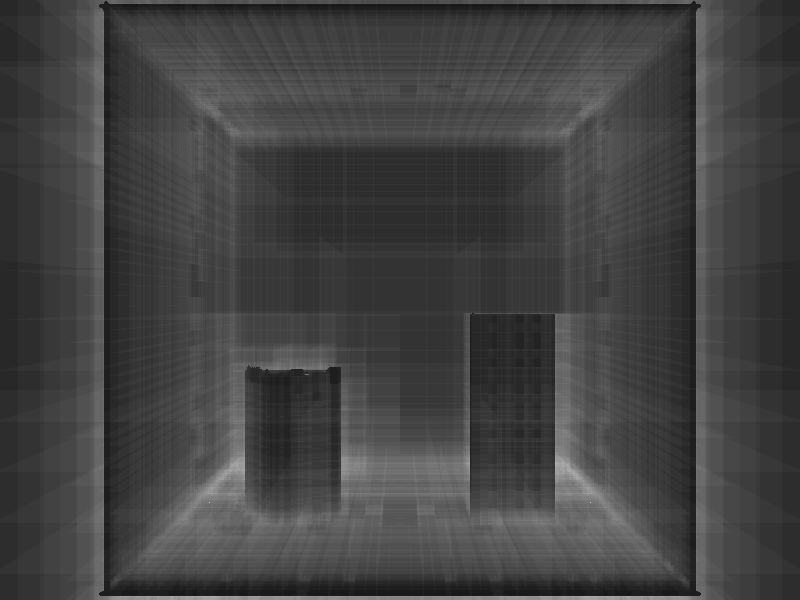
\includegraphics[width=100mm]{img/testing.png}
    \caption{Illustrates the octree traversal algorithm testing efficiency.  Lighter shades represent less tests, while darker shades represents the most.  Closer objects evaluate faster, and all data in the point-cloud behind them are occluded.}
    \label{fig:testing}
\end{figure}

%------------------------------------------------------------%
\subsection{Acquiring Scatter-Out Contributions}
\label{scatterout_sec}

Once the changes to the point-cloud data-structure have been made, we are able to 1) guarantee correct evaluation of the transparent surfaces through front-to-back octree traversal and 2) stop evaluating leaf nodes once we have hit an opaque surfel, reducing the overall sample count.  Now that \textit{lvoxels} are supported, we simply sample the scene as we have with regular PCB.  The modified traversal algorithm already takes care of transmittance through any transparent media so no further changes are necessary.

%------------------------------------------------------------%
\subsection{Acquiring Scatter-In Contributions}
\label{scatterin_sec}
After adding lvoxels to our octree structure and evaluation algorithm, the only modifications necessary for scatter-in are to the volume rendering equation.  As an overview, volume integration will step through the volume, at each point it will:

\begin{enumerate}
\item Update the current transmittance by the scatter and absorption terms at the given point
\item Cast shadow rays to estimate the direct light (and in cases of non-uniform scatter, apply a phase function)
\item Sample scatter contribution by sending rays out into the point cloud
\item Add direct illumination contribution and indirect illumination to the current incoming radiance
\end{enumerate}

Recall that to model lighting for a volume, in-scattering requires integrating over all directions.  Casting Monte Carlo sample rays through the volume and into the scene would be computationally expensive.  Instead, for each sample we send out rays into the point cloud, iterating through a much less dense dataset like in Figure \ref{fig:scatter_in}.

This method helps us replace expensive $S(\textup{p, w})$ evaluations with traversals into the octree.  The two main differences between sampling scattered light within a volume and evaluating the irradiance on a surface are 1) the distribution function, which is based on the volume's phase function, and 2) the samples are distributed over a sphere rather than a hemisphere.

These scatter samples are distributed throughout the volume marching process typically taken while rendering volumes as seen in Figure \ref{fig:vol_step}.  The ray generates a series of sample points through the volume and iterates through, gathering light from direct lighting and indirect sampling as well as updating the ray's transmittance (which identifies how much light passes through the volume from behind.)


\begin{figure}[h!]
    \centering
    \includegraphics[width=80mm]{img/diag/scatter_in.pdf}
    \captionfonts
    \caption{Sample rays are cast during volume traversal, allowing for decent estimates of lighting contribution at each point.}
    \label{fig:scatter_in}
\end{figure}


\begin{figure}[h!]
    \centering
    \includegraphics[width=80mm]{img/diag/vol_step.pdf}
    \captionfonts
    \caption{Stepping allows for estimation of the integral through the entire volume.  Shadow rays are cast intermittently to estimate the direct lighting contribution. }
    \label{fig:vol_step}
\end{figure}

%==============================================================================%
\chapter{Results}

This section will discuss the testing environment and test scenario used to compare traditional Monte Carlo gather methods with the results that we were able to achieve using our PCB Extension algorithm.

\begin{figure}[h!]
    \centering
    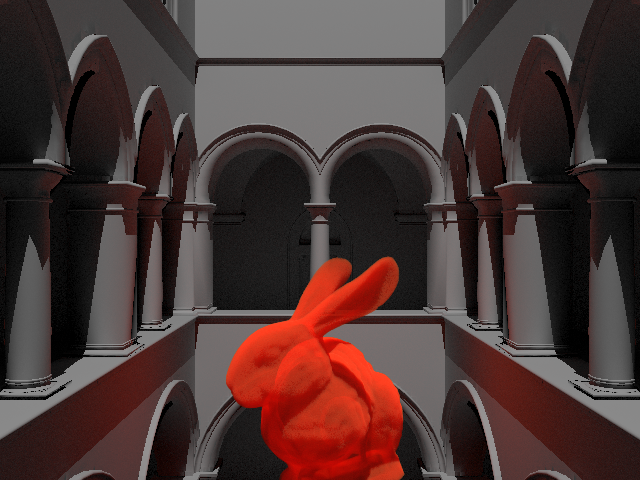
\includegraphics[width=120mm]{img/sponza.png}
    \caption{Sponza Atrium mesh and Stanford bunny volume rendered using the PCB Extension algorithm.}
    \label{fig:sponza_results}
\end{figure}

\begin{figure}[h!]
\centering
    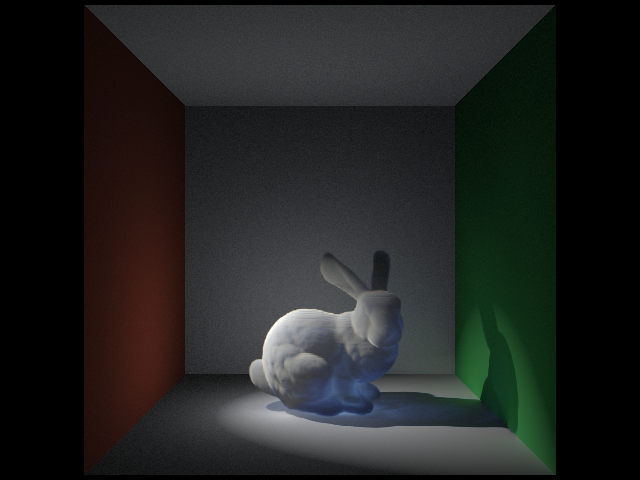
\includegraphics[width=60mm]{img/bunny_spot/spot_left.png}
    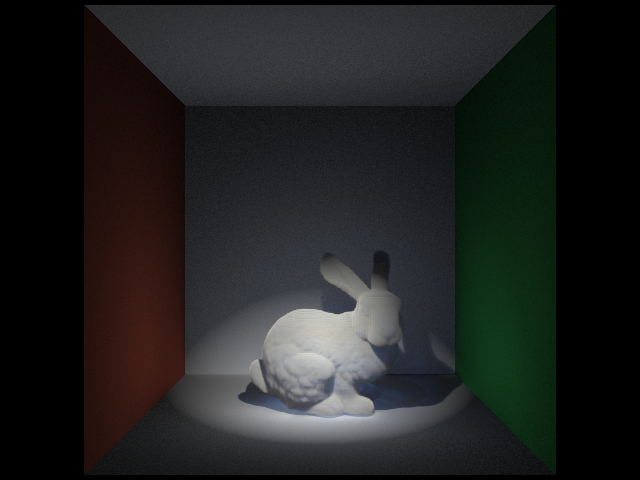
\includegraphics[width=60mm]{img/bunny_spot/spot_front.png}

    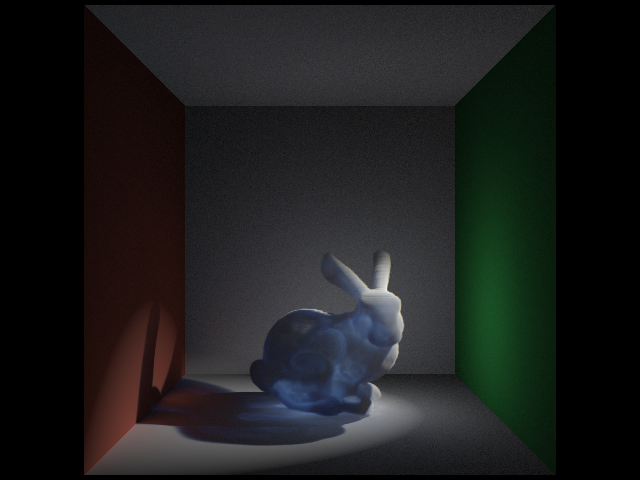
\includegraphics[width=60mm]{img/bunny_spot/spot_right.png}
    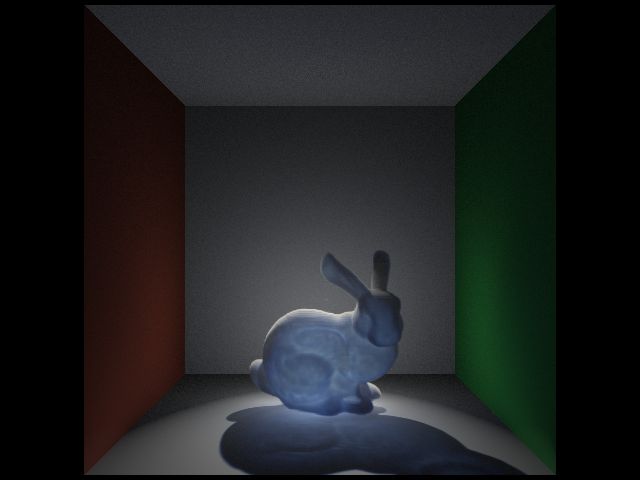
\includegraphics[width=60mm]{img/bunny_spot/spot_behind.png}
    \captionfonts
    \caption{A test scene showing a light's interaction with a volume changing depending on the direction and position of the light.}
\end{figure}

\section{Environment}

Our algorithm is able to achieve realistic lighting effects for scenes that include volumetric elements using our lvoxel representation with a point-based color bleeding approach to global illumination.
The following test cases were run on a commodity-class Intel i5 3 GHz machine with 4 Gb of RAM.  Because of the disparity between academic-level versus production-class ray tracer implementations, we tested and compared our results against a naive implementation of Monte Carlo global illumination not using the point cloud representation.  We then compared the resulting images and the time it took to render each.  Our algorithm is able to achieve a small difference between images and an increase in efficiency measured in time to render.

\section{Test Scene}

\begin{figure}[h!]
    \centering
    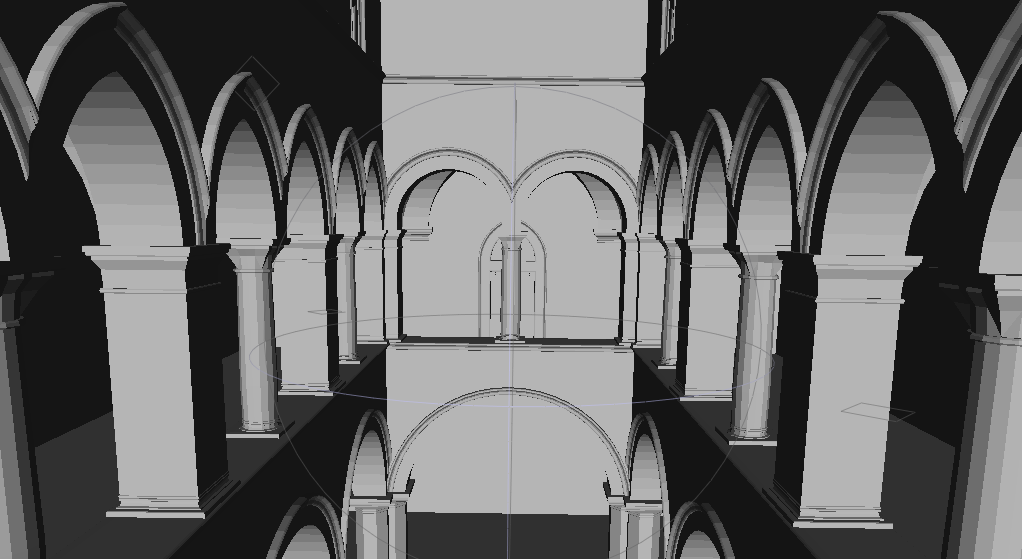
\includegraphics[width=120mm]{img/sponza_vis.png}
    \captionfonts
    \caption{Real-time visualization of the Sponza Atrium mesh in MeshLab.}
    \label{fig:inscat}
\end{figure}

The scene tested involved a 60,000 triangle Sponza Atrium including only vertex and normal information for simplicity.  The CT scan data of the Stanford Bunny was used in order to test scatter in/out contributions by complex participating media.
Figure~\ref{fig:compare} shows the bunny and Sponza Atrium showing traditional Monte Carlo scattering.  At first glance these two images are very similar, however there are a number of small artifacts present in the image rendered with the point cloud representation, and the indirect lighting is slightly darker overall.  A closer look at the two results exemplifies the great similarity between the two images, as shown in Figure~\ref{fig:compare_close}.

Every test rendered a 640x480 image with 128 light samples per ray.

%------------------------------------------------------------%
\section{Data Comparison}

\begin{center}
\setlength{\tabcolsep}{5pt}
\begin{tabular}{ | l | c | c | c | }
  \hline                       
  Scene & Render Time (s) & Image Delta & Memory Overhead \\
  \hline                  
  Monte Carlo w/o PCB & 3351 sec & NONE & NONE \\
  Traditional PCB & 348 sec & 11.0\% & 390 Mb (4.0\%) \\
  Extended PCB & 397 sec & 4.8\% & 395 Mb (4.1\%)  \\
  \hline  
\end{tabular}
\label{Data Comparison}
\end{center}


%------------------------------------------------------------%
\section{Analysis}
Our analysis involves comparing 1) the overall render time 2) the perceived image delta between the images and 3) the memory overhead used by the point-cloud data.

%----------------------------------%
\subsection{Memory}
When using traditional PCB, the real benefit to its surfel representation is shown in more complex scenes.  In the Sponza Atrium, the scene generated over 2.5 million surfels for a 60,000 triangle scene.  Adding volume data to the scene does not add an objectionable amount of data to the point cloud, but for scenes with large volumes the costs could quickly add up without some form of multi-resolution light caching.  In this regard, adding yet another representation of the volumes may be expensive, but not prohibitively so.  Additionally, larger scenes would benefit from this representation, as it would be significantly simpler than the entire scene and can be moved to another system for out-of-core evaluation.

%----------------------------------%
\subsection{Speed}
Even without volume integration, Monte Carlo integration without a lighting representation like PCB is prohibitively slow for even the simplest scenes.  Adding a point cloud representation gave us an impressive speedup.  That speedup was compounded even more when volume scattering was added into the tests, showing a factor of eight speedup for our test scenes.

Even on sparse octrees without volumes, our \textit{front to back} octree traversal method operates at an efficiency of $O\log{n}$ for each node traversal while skipping nodes occluded by surfels, leading to an average performance increase of over 18\%.

%----------------------------------%
\subsection*{Image Quality}

In order to objectively compare the pure Monte Carlo render to the PCB extension render, we used a perceptual image difference program called pdiff and ran the pair of images through in order to identify how close the two images were to each other.  The results showed a clear difference (where pixels in one image clearly different from another) of 4.8\%.


\begin{figure}[h!]
    \centering
    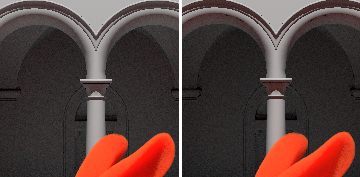
\includegraphics[width=80mm]{img/compare1_corrected.png}
    \captionfonts
    \caption{Zoomed image showing PCB extension (left) and Monte Carlo (right.)}
    \label{fig:compare_close}
\end{figure}

\begin{figure}[h!]
    \centering
    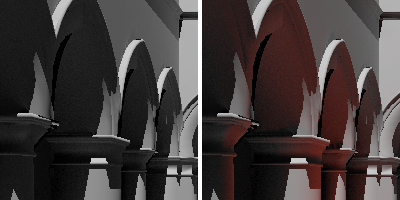
\includegraphics[width=80mm]{img/compare_trad_corrected.png}
    \captionfonts
    \caption{Zoomed image showing traditional PCB (left) and PCB with extension (right.)  Note the visible color bleeding with our method.}
    \label{fig:compare_trad}
\end{figure}

Figure~\ref{fig:compare_trad} compares the non-PCB Monte Carlo image with that of the traditional PCB renders, showing the clear lack of proper in-/out-scattering.  With the extended algorithm, however, the scenes look nearly identical.

We would like to note that there are a number of small artifacts in the PCB renders due to imprecision and incorrect surfel collisions.  It is important to note that, as past papers will attest, such issues are easily overcome and our artifacts are more due to implementation and time constraints than limits on the algorithm itself.

\section{Conclusion}

In this paper, we discussed the necessity for proper global illumination approximations in renders, listed a number of algorithms that have attempted to do this but have fallen short specifically in volume scatter contributions, and presented an extension to the PCB algorithm by \cite{christensen:2008} which handles both scatter-in and scatter-out contributions.  The addition of the lvoxel paradigm to the already successful point based color bleeding algorithm is shown to be a cost effective method of approximating and evaluating complex scatter functions based on participating media.  The speedups are clear, and the memory footprint is easily manageable.  The ability to evaluate the irradiance at a point in the scene by using only the point cloud representation is a clear win for out-of-core renderers.

Computer graphics, be it photo-realistic or artistically leaning, relies heavily on the paradigms established in the physics of light in the real world.  Global illumination is just one of many areas of focus trying to better represent that light and its complex interactions in the abstract worlds we choose to bring to screen.  One can only imagine the leaps and bounds that computer graphics is destined to experience in the following years, but inevitably the obstacles boil down to the same subset of problems.  How to manipulate light and, by extension, color in order to make the viewer experience a story or emotion.

%==============================================================================%
\chapter{Future Work}


As mentioned in Christensen's point based color bleeding article, surfels can be modified to ``gather'' light recursively from their position in the point cloud, allowing for simulated multi-bounce lighting.  This would require only a small change to the current algorithm, and would apply to volumes as well to allow very realistic scatter approximations in participating media.

\vspace{5mm}

In our tests, all participating media scatters light equally in all directions.  This is rarely the case, as volumes tend to have unique scatter functions.  We can simulate more complex surface scattering functions by creating spherical harmonic representations of the radiance at any specific point in the volume.  Our current implementation supports such an approach, but remains untested.

\vspace{5mm}

Typical implementations of the PCB algorithm include rougher estimations (usually in the form of a series of spherical harmonic coefficients) at higher levels in the octree, to be evaluated depending on that node's solid angle to our sample point.  Due to time constraints, we did not implement full multi-resolution representations of each node.  Including LVoxel data in that representation would be a trivial process.

\vspace{5mm}

Our ray tracer runs a number of threads to split the image into multiple parts  in order to achieve simple parallelism.  Before the threads are created, however, we generate surfels and lvoxels sequentially.  Due to the nature of our octree implementation, we cannot add elements and still be thread safe, but this would not be a large obstacle.  Scenes like the sponza atrium would run a number of times faster if we were to parallelize our implementation more effectively.

\vspace{5mm}

Although for our purposes ray casting the scene to sample for surfels worked well, it is most certainly not an optimal algorithm.  Sampling the scene in a more geometry- aware fashion would lead to fewer samples and better results.  Subdividing the scene into smaller polygons and sampling the scene (say, one or two surfels per micro-polygon) would increase our coverage while decreasing unnecessary overlap.  We found that the simpler approach worked best for us, given our time frame, however it can most certainly be improved.

\vspace{5mm}

Because the color-bleeding effect in PCB focuses primarily on the point-cloud data, we are offered a unique opportunity to consider offloading the entire octree structure out-of-core in order to outsource the (still computationally complex) algorithm onto other machines, if not to on-board GPUs.  Taking advantage of a graphics processor's fast math and hardware rasterization would allow for much faster indirect-lighting evaluations.

% ------------- End main chapters ----------------------

\clearpage
\bibliography{pcbex}
\bibliographystyle{plain}
%\addcontentsline{toc}{chapter}{Bibliography}



%==============================================================================%

\section*{Image Results}

\begin{figure}[h!]
    \centering
    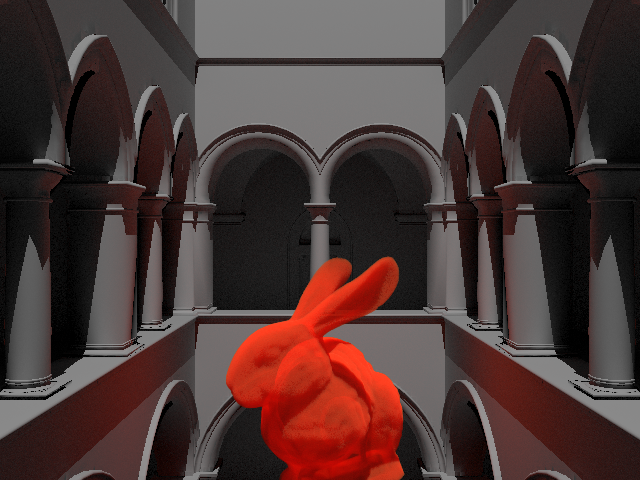
\includegraphics[height=90mm]{img/sponza.png}
    \captionfonts
    \caption{The Sponza Atrium with the Stanford volumetric bunny.  In-/Out-scattering is evident on the volume and on the surrounding atrium walls.}
\end{figure}

\begin{figure}[h!]
    \centering
    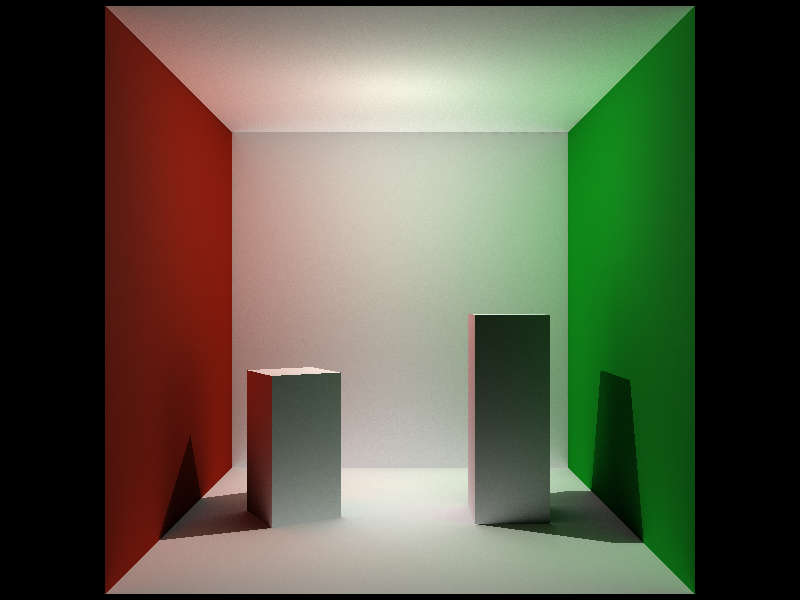
\includegraphics[height=90mm]{img/indirect_box_high.png}
    \captionfonts
    \caption{Example of point-based color bleeding without the volume extension algorithm.}
\end{figure}

\begin{figure}[h!]
    \centering
    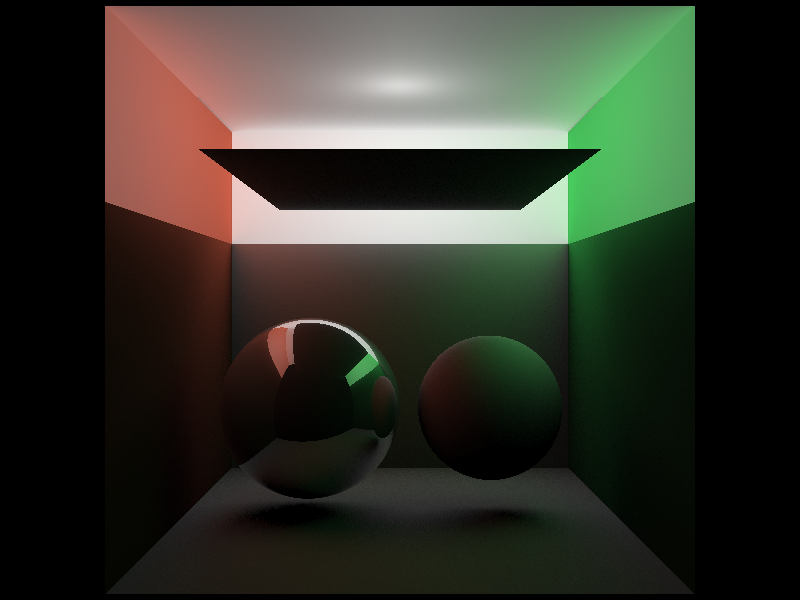
\includegraphics[height=90mm]{img/two_sphere_indir.png}
    \captionfonts
    \caption{Example of a scene almost entirely in shadow, showing indirect lighting in play.}
\end{figure}

\begin{figure}[h!]
    \centering
    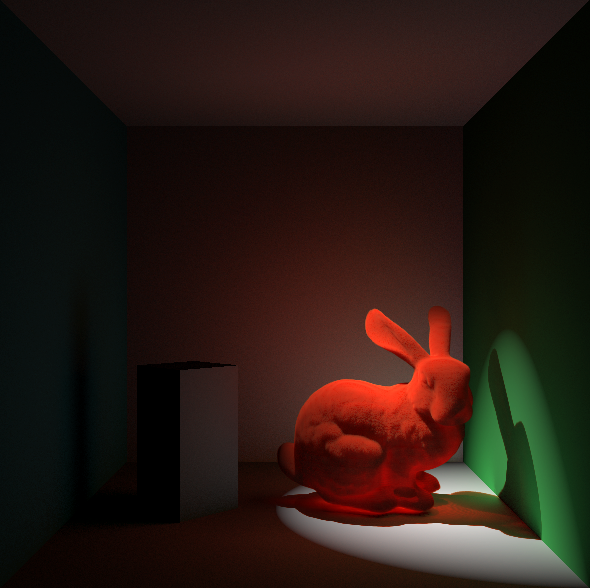
\includegraphics[height=90mm]{img/ketchup_good_corrected.png}
    \captionfonts
    \caption{Image exemplifying clear out-scattering from Stanford bunny volume.}
\end{figure}

\begin{figure}[h!]
    \centering
    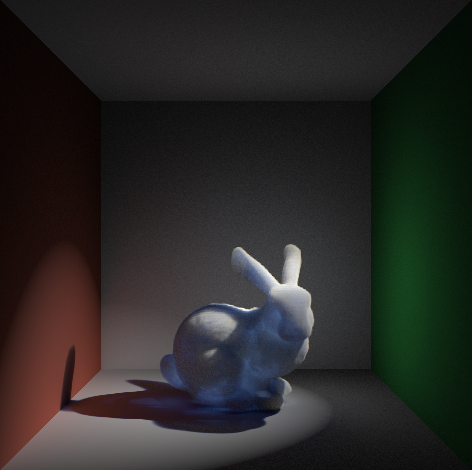
\includegraphics[height=90mm]{img/bunny_spot/spot_right_new.png}
    \captionfonts
    \caption{Image exemplifying clear color bleeding next to the red wall in the bunny's shadow and correct transmittance through the bunny's hollow form.}
\end{figure}

\begin{figure}[h!]
    \centering
    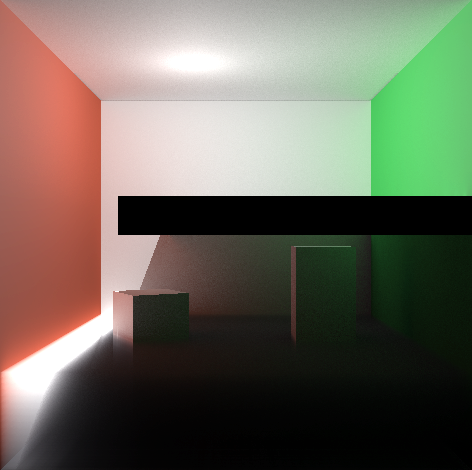
\includegraphics[height=90mm]{img/one_side_corrected.png}
    \captionfonts
    \caption{The black occluding geometry in the center stops all but the light to the left to enter below.}
\end{figure}

\begin{figure}[h!]
    \centering
    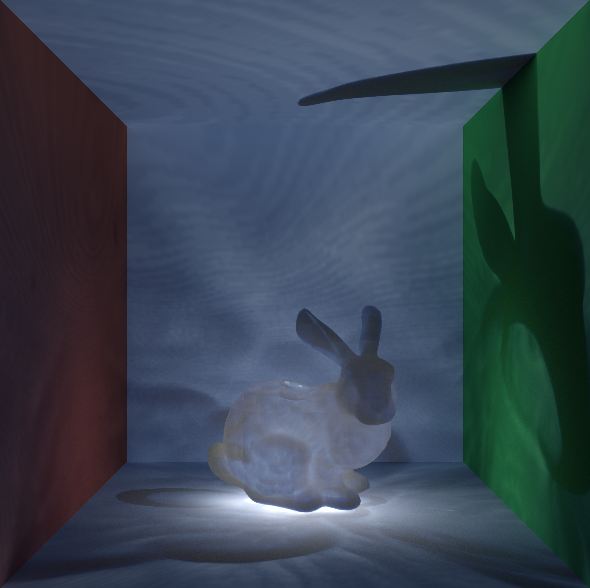
\includegraphics[height=90mm]{img/bunny_glow.png}
    \captionfonts
    \caption{Illustrates how a light may act when placed within a hollow volumetric object.  The bunny is shown as slightly brighter, scattering light about the scene.}
\end{figure}

\begin{figure}[h!]
    \centering
    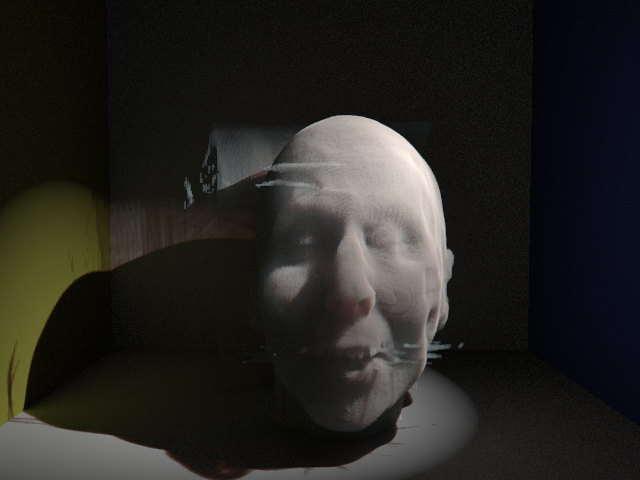
\includegraphics[height=90mm]{img/face1.png}
    \captionfonts
    \caption{Shows how CT scan data can be used to visualize scanned objects like a human face.  Subsurface scattering and transmittance through thin materials is evident.}
\end{figure}



\end{document}
